\documentclass[xcolor=pdflatex,dvipsnames,table]{beamer}
\usepackage{epsfig,graphicx}
\usepackage{palatino}
\usepackage{fancybox}
\usepackage{relsize}
\usepackage[procnames]{listings}
\usepackage{hyperref}
\usepackage{qtree} % needed?
\usepackage{booktabs}
\usepackage{dirtree}
\usepackage[normalem]{ulem}


% fatter TT font
\renewcommand*\ttdefault{txtt}
% another TT, suggested by Alex
% \usepackage{inconsolata}
% \usepackage[T1]{fontenc} % needed as well?


\newcommand{\scale}{0.7}

\newcommand{\todo}[1]{{\emph{TODO: #1}}}
\newcommand{\martin}[1]{{\color{blue} Martin: #1}}
\newcommand{\abcdef}[1]{{\color{red} Author2: #1}}

% uncomment following for final submission
%\renewcommand{\todo}[1]{}
%\renewcommand{\martin}[1]{}
%\renewcommand{\author2}[1]{}

\newcommand{\code}[1]{{\texttt{#1}}}

\hypersetup{
  linkcolor  = black,
%  citecolor  = blue,
  urlcolor   = blue,
  colorlinks = true,
}

\beamertemplatenavigationsymbolsempty
\setbeamertemplate{footline}[frame number]





\newif\ifbook
% shared in slides and book

\lstdefinelanguage{chisel}{
%  morekeywords={abstract,case,catch,class,def,%
%    do,else,extends,false,final,finally,%
%    for,if,implicit,import,match,mixin,%
%    new,null,object,override,package,%
%    private,protected,requires,return,sealed,%
%    super,this,throw,trait,true,try,%
%    type,val,var,while,with,yield},
%  otherkeywords={=>,<-,<\%,<:,>:,\#,@},
  sensitive=true,
  morecomment=[l]{//},
  morecomment=[n]{/*}{*/},
  morestring=[b]",
  morestring=[b]',
  morestring=[b]"""
}

\usepackage{color}
\definecolor{dkgreen}{rgb}{0,0.6,0}
\definecolor{gray}{rgb}{0.5,0.5,0.5}
\definecolor{mauve}{rgb}{0.58,0,0.82}

% Default settings for code listings
%\ifbook
\lstset{%frame=lines,
  language=chisel,
  aboveskip=3mm,
  belowskip=3mm,
  showstringspaces=false,
  columns=fixed, % basewidth=\mybasewidth,
  basicstyle={\small\ttfamily},
  numbers=none,
  numberstyle=\footnotesize,
  % identifierstyle=\color{red},
  breaklines=true,
  breakatwhitespace=true,
  procnamekeys={def, val, var, class, trait, object, extends},
  % procnamestyle=\ttfamily,
  tabsize=2,
  float
}
%\else
%\lstset{%frame=lines,
%  language=chisel,
%  aboveskip=3mm,
%  belowskip=3mm,
%  showstringspaces=false,
%  columns=fixed, % basewidth=\mybasewidth,
%  basicstyle={\small\ttfamily},
%  numbers=none,
%  numberstyle=\footnotesize\color{gray},
%  % identifierstyle=\color{red},
%  keywordstyle=\color{blue},
%  commentstyle=\color{dkgreen},
%  stringstyle=\color{mauve},
%  breaklines=true,
%  breakatwhitespace=true,
%  procnamekeys={def, val, var, class, trait, object, extends},
%  procnamestyle=\ttfamily\color{red},
%  tabsize=2,
%  float
%}
%\fi

\lstnewenvironment{chisel}[1][]
{\lstset{language=chisel,#1}}
{}

\newcommand{\shortlist}[1]{{\lstinputlisting[nolol]{#1}}}

\newcommand{\longlist}[3]{{\lstinputlisting[float, caption={#2}, label={#3}, frame=tb, captionpos=b]{#1}}}

\newcommand{\verylonglist}[3]{{\lstinputlisting[caption={#2}, label={#3}, frame=tb, captionpos=b]{#1}}}


\title{Software-Defined Hardware: Digital Design in the 21st Century with Chisel}
\author{Martin Schoeberl}
\date{\today}
\institute{Technical University of Denmark}

\begin{document}

\begin{frame}
\titlepage
\end{frame}

%\begin{frame}[fragile]{Welcome}
%\begin{itemize}
%\item You can also join this session via the Zoom app
%\item Probably better quality and more functions
%\item The link is in the Whova chat
%%\item \url{https://dtudk.zoom.us/j/61032875012}
%%\item Let us have an introduction round
%\item This shall be interactive: please join with video!
%\item You can ask questions by unmuting and just talking
%\item Use the chat in Zoom to ask questions
%\end{itemize}
%\end{frame}

\begin{frame}[fragile]{TODO}
\begin{itemize}
\item Chisel for engineers who now V*
\item Just 2 slides on the Chisel syntax for wires, register, and modules
\item Focus on advanced material
\item real generics (Mux)
\item Object oriented (FIFO example)
\item Flip for one definition
\item \code{<>} for connecting those elements (P, FIFO, C)
\item Full Java/Scala world available, show Basys 3 simulation
\item Functional programming for circuit generators
\item Arbiter from simple arbiters
\item Look into Scott's examples
\end{itemize}
\end{frame}

\begin{frame}[fragile]{Motivating Example:\\
Lipsi: Probably the Smallest Processor in the World}
\begin{itemize}
\item Tiny processor
\item Simple instruction set
\item Shall be small
\begin{itemize}
\item Around 200 logic cells, one FPGA memory block
\end{itemize}
\item Hardware described in Chisel
\item Available at \url{https://github.com/schoeberl/lipsi}
\item Usage
\begin{itemize}
\item Utility processor for small stuff
% \item Could be used for your vending machine
\item In teaching for introduction to computer architecture
\end{itemize}
\item The design took place on the island Lipsi
\end{itemize}
\end{frame}

\begin{frame}[fragile]{The Design of Lipsi on Lipsi}
\begin{figure}
    \centering
    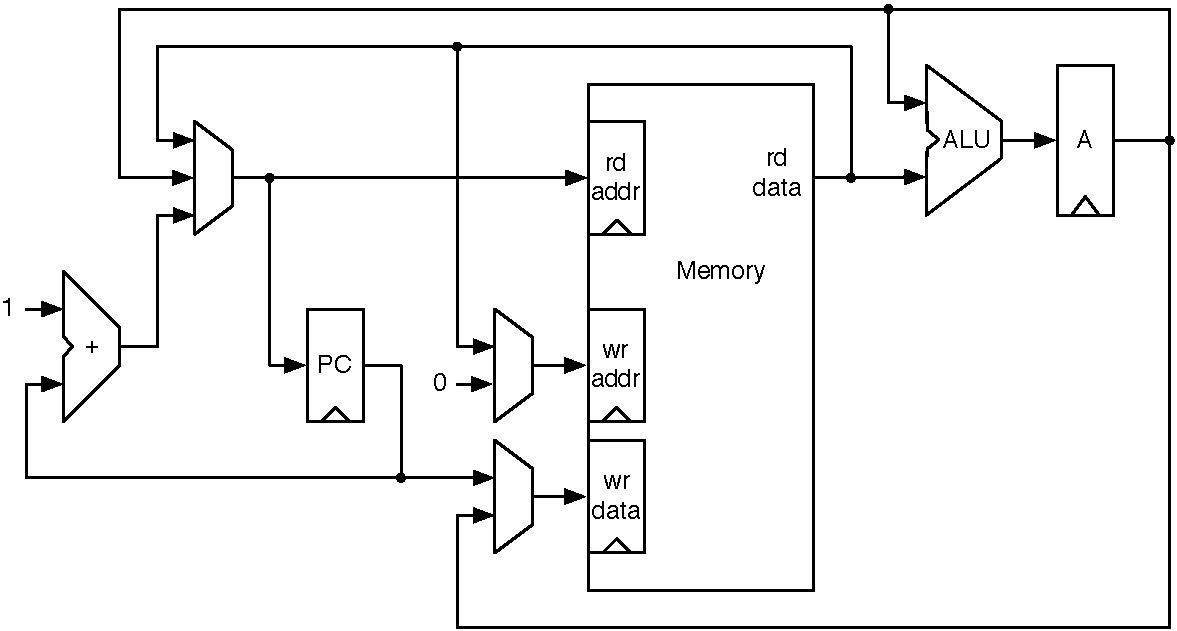
\includegraphics[scale=0.3]{lipsi}
\end{figure}
\end{frame}

\begin{frame}[fragile]{Lipsi Implementation}
\begin{itemize}
\item Hardware described in Chisel
\item Tester in Chisel
\item Assembler in Scala
\begin{itemize}
\item Core case statement about 20 lines
\end{itemize}
\item Reference design of Lipsi as software simulator in Scala
\item Testing:
\begin{itemize}
\item Self testing assembler programs
\item Comparing hardware with a software simulator
\end{itemize}
\item All in a single programming language!
\item All in a single program
\item How much work is this?
\end{itemize}
\end{frame}

\begin{frame}[fragile]{Chisel is Productive}
\begin{itemize}
\item All coded and tested in less than 14 hours!
\end{itemize}
\begin{itemize}
\item The hardware in Chisel
\item Assembler in Scala
\item Some assembler programs (blinking LED)
\item Simulation in Scala
\item Two testers
\end{itemize}
\begin{itemize}
\item BUT, this does not include the design (done on paper)
\end{itemize}
\end{frame}

\begin{frame}[fragile]{Motivating Example: Lipsi, a Tiny Processor}
\begin{itemize}
\item Show in IntelliJ
\end{itemize}
\end{frame}

%\begin{frame}[fragile]{The Slides are Online}
%\begin{itemize}
%\item \url{https://github.com/schoeberl/chisel-book/wiki}
%\end{itemize}
%\begin{figure}
%    \centering
%    \includegraphics[scale=0.5]{slides-link}
%\end{figure}
%\end{frame}

\begin{frame}[fragile]{More on Chisel Success Stories}
\begin{itemize}
\item Before the lockdown at CCC 2020 (in silicon valley)
\item 90 participants
\item More than 30 different (hardware) companies present
\item Several companies are looking into Chisel
\item IBM did an open-source PowerPC
\item \href{https://www.sifive.com/}{SiFive} is a RISC-V startup success
\begin{itemize}
\item High productivity with Chisel
\item Open-source Rocket chip
\end{itemize}
\item Experanto uses the BOOM processor in Chisel
\item Google did a machine learning processor
\item Intel is looking at Chisel
\item Chisel is open-source, if there is a bug you can fix it
\begin{itemize}
\item You can contribute to the Chisel ecosystem
\end{itemize}
\end{itemize}
\end{frame}

\begin{frame}[fragile]{Goals for this Intro}
\begin{itemize}
\item Get an idea what Chisel is
\begin{itemize}
\item Will show you code snippets
\end{itemize}
\item TODO: adapt
\end{itemize}
\end{frame}


\begin{frame}[fragile]{Chisel}
\begin{itemize}
\item A hardware \emph{construction} language
\begin{itemize}
\item Constructing Hardware In a Scala Embedded Language
\item If it compiles, it is synthesisable hardware 
\item Say goodby to your unintended latches
\end{itemize}
\item Chisel is not a high-level synthesis language
\item Single source two targets
\begin{itemize}
\item Cycle accurate simulation (testing)
\item Verilog for synthesis
\end{itemize}
\item Embedded in Scala
\begin{itemize}
\item Full power of Scala available
\item But to start with, no Scala knowledge needed
\end{itemize}
\item Developed at UC Berkeley
\item Drives the Rocket chip (open-source RISC-V)
\end{itemize}
\end{frame}



\end{document}

\begin{frame}[fragile]{Title}
\begin{itemize}
\item abc
\end{itemize}
\end{frame}
